\section{Programming Abstractions and Constraints for NPU Kernel Generation}
\label{sec:programming_constraints}

\begin{comment}

\subsection{Ascend NPU: DaVinci Architecture}
\label{sec:hardware_arch}

The Ascend 910B1 NPU leverages the advanced DaVinci architecture, characterized by a decoupled heterogeneous computing paradigm that physically segregates matrix and vector processing to maximize computational efficiency. As illustrated in Figure~\ref{fig:NPU}, where arrows denote the directional data processing flow, the architecture is fundamentally divided into two independent execution engines: the Matrix Computation Engine (AI Cube, or AIC) and the Vector Computation Engine (AI Vector, or AIV). To achieve massive parallelism, each NPU integrates 25 AICs and 50 AIVs, culminating in a peak computing performance of 379 TFLOPS in FP16 precision.

The AIC (top section) is specialized for high-throughput tensor operations, employing a hierarchical memory structure managed by dedicated Memory Transfer Engines (MTE1/MTE2/MTE3). Data is prefetched from Global Memory (GM) into an on-chip L1 Buffer and subsequently distributed to Buffer L0A and Buffer L0B to feed the CUBE unit for matrix multiplication, with results accumulated in Buffer L0C. The architecture incorporates specialized on-chip storage to accelerate post-processing: the BT Buffer is designated for storing bias values, while the Fixpipe Buffer holds quantization and ReLU parameters. Conversely, the AIV (bottom section) handles complex element-wise and scalar logic, centered around a massive Unified Buffer (UB) that serves both the Scalar Unit and the Vector Unit. A critical feature of this split-core design is the independence of the instruction streams; the AIC and AIV can load separate code segments and execute asynchronously, coupled only by data exchange through the Global Memory. This decoupling allows for fine-grained software scheduling, enabling the massive parallelism of the Cube units to operate concurrently with the flexible logic of the Vector units, thereby optimizing the overall throughput for diverse deep learning workloads.

\begin{figure}[t]
    \centering
    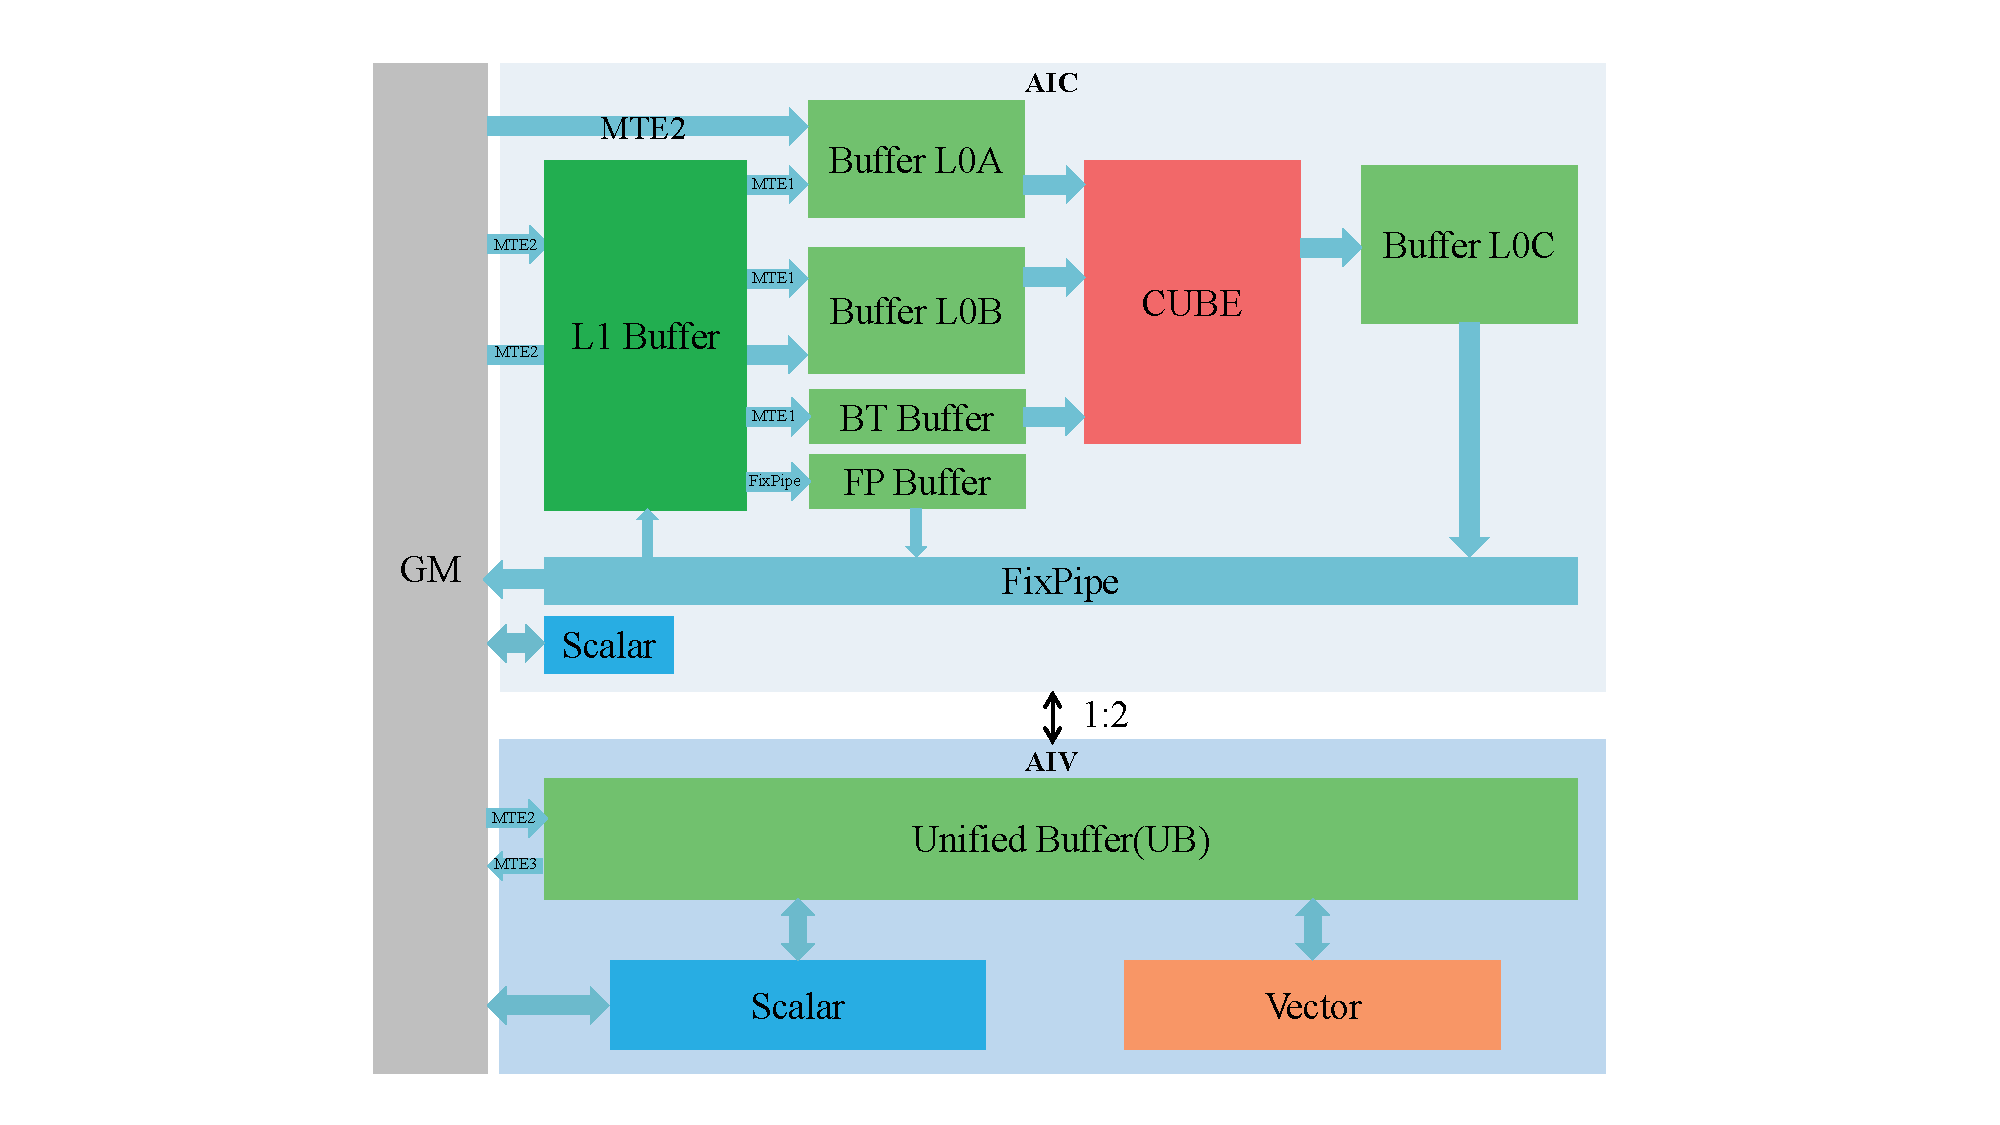
\includegraphics[width=0.6\linewidth, trim={6.4cm 1.0cm 6.6cm 1.0cm}, clip]{pdfs/910B.pdf}
    \caption{DaVinci architecture of Huawei Ascend 910B1 NPU}
    \label{fig:NPU}
\end{figure}

\subsection{Ascend Programming Model: SPMD and Pipeline Parallelism}
\label{sec:programming_model}

To abstract the complexity of the underlying heterogeneous hardware while exposing its massive parallelism, the Ascend processor employs a programming model characterized by Single-Program Multiple-Data (SPMD) execution and Asynchronous Pipeline Parallelism. This model provides the necessary structural template that our generation framework follows.

\paragraph{SPMD Execution Paradigm}
The Ascend NPU adopts the SPMD model to scale computational throughput. A single kernel function is instantiated across multiple AI Cores simultaneously. All cores execute the exact same instruction stream, but operate on disjoint data partitions. The distinction is managed via a unique logical index (\texttt{block\_idx}), which the generated code must use to calculate memory offsets for global data slicing. This paradigm allows the LLM to focus on generating the logic for a single data block, while the hardware handles the massive parallel dispatch.

\paragraph{Asynchronous Pipeline Parallelism}
To mask the latency difference between the Memory Transfer Engines (MTEs) and the Computation Units (Vector/Cube), the programming model enforces a strict pipeline paradigm. As depicted in the standard flow, a kernel task is decomposed into three asynchronous stages:
\begin{enumerate}
    \item CopyIn: Moves data from high-latency Global Memory (GM) to on-chip Local Memory (e.g., Unified Buffer or L1).
    \item Compute: Performs vector or matrix operations on the on-chip data.
    \item CopyOut: Writes the results back to Global Memory.
\end{enumerate}
These stages execute on independent hardware units. By organizing the code into a multi-stage pipeline, the NPU can overlap the computation of the current data block with the data prefetching of the next block, achieving high pipeline efficiency.

\paragraph{Resource Abstraction and Synchronization}
To manage the on-chip resources and dependencies within this pipeline, the model introduces high-level abstractions:
\begin{itemize}
    \item Logical Storage (TPosition): Physical memory hierarchies are abstracted into logical positions. This relieves the generator from managing physical addresses, allowing it to focus on data flow logic.
    \item Queue-based Synchronization (TQue): To resolve Read-After-Write (RAW) and Write-After-Read (WAR) dependencies between asynchronous stages, the model utilizes a queue-based mechanism. The \texttt{EnQue} operation signals data production, while \texttt{DeQue} signals data consumption. Correctly pairing these operations allows the underlying hardware to automatically enforce synchronization barriers without explicit low-level programming.
\end{itemize}

In summary, for an LLM to generate valid Ascend kernels, it must adhere to this specific structure: implementing the logic within an SPMD context, organizing operations into a CopyIn-Compute-CopyOut pipeline, and utilizing TQue interfaces to ensure memory consistency.

\subsection{Hierarchical API Architecture and Generation Challenges}
\label{sec:api_architecture}

Ascend C provides a multi-level API hierarchy that abstracts hardware intrinsics into standard C++ interfaces.  While this architecture includes both High-Level and Basic APIs, automatic kernel generation utilizing Basic APIs represents the primary challenge and value proposition for LLM-based research.

\paragraph{High-Level APIs (Algorithmic Abstractions)}
This layer encapsulates common compute-intensive patterns (e.g., \texttt{Matmul}, \texttt{Softmax}) into object-oriented classes. By internalizing the complex pipeline logic and tiling strategies, these APIs serve as "black-box" solutions. While convenient, they lack the flexibility required for implementing novel or non-standard operators, limiting the scope of LLM generation to a fixed set of predefined algorithms.

\paragraph{Basic APIs (The Focus of Generation)}
To achieve true programmability and support arbitrary custom operators, LLMs must master the Basic APIs, which provide granular control over the hardware. This layer serves as a direct abstraction of the Instruction Set Architecture (ISA) and comprises:
\begin{itemize}
    \item Computation Primitives: Interfaces for invoking specific execution units, such as Vector (SIMD) and Cube (Matrix) operations.
    \item Explicit Pipeline Management: Unlike High-Level APIs, Basic APIs require the programmer (or LLM) to manually manage the data movement (via \texttt{DataCopy}) and inter-stage synchronization (via \texttt{EnQue}/\texttt{DeQue}).
    \item High-Dimensional Slicing: Vector computation APIs support complex addressing patterns via sophisticated parameters like \texttt{mask}, \texttt{repeatStride}, and \texttt{dataBlockStride}. This enables non-contiguous data processing within a single instruction but imposes significant logical complexity.
\end{itemize}

\paragraph{Challenges for LLM Generation}
By targeting the flexible Basic APIs rather than the rigid High-Level ones, the generation task shifts from simple API calls to complex low-level systems programming, introducing distinct challenges:

\begin{enumerate}
    \item Manual Pipeline Orchestration: The LLM cannot rely on automatic scheduling. It must act as a compiler to manually weave computation with synchronization logic. It must strictly adhere to the resource lifecycle—\texttt{AllocTensor} $\to$ \texttt{EnQue} $\to$ \texttt{DeQue} $\to$ \texttt{FreeTensor}—to prevent memory leaks or execution deadlocks. This demands a deep understanding of the hardware's asynchronous nature, which is often absent in general-purpose training data.
    
    \item Precise Mathematical Reasoning for Tiling: Configuring Basic APIs requires calculating intricate stride and mask parameters to handle data alignment and tail blocks. For instance, determining the correct \texttt{mask} (bit-level control) or \texttt{repeatStride} (inter-iteration gaps) requires precise arithmetic reasoning. A minor calculation error by the LLM leads to silent data corruption or hardware exceptions.
    
    \item Hardware-Aware Vectorization: The model must generate SPMD-friendly code. This involves understanding the NPU's data alignment requirements (e.g., 32-byte alignment for Unified Buffer access) and effectively utilizing the massive parallelism of the Cube/Vector unit.
\end{enumerate}


\subsection{Implementation Paradigms and Generation Challenges on Ascend NPU}
\label{sec:implementation_challenges}

Implementing high-performance operators on the Ascend NPU adheres to a rigorous heterogeneous computing paradigm. While sharing commonalities with other accelerators (e.g., explicit memory hierarchies), Ascend C enforces a distinct development pattern, particularly in how tiling strategies and pipeline synchronization are architected. These constraints present specific reasoning challenges for Large Language Models (LLMs).

\paragraph{Host-Centric Tiling Calculation}
Unlike typical CUDA kernels where tiling offsets and loop bounds are often calculated dynamically on the device (using thread indices), Ascend C architecturally enforces the offloading of Tiling Logic to the Host. The Host calculates complex parameters (e.g., block sizes, tail offsets, iteration counts) based on the input shape, while the Device kernel acts purely as a consumer of these pre-computed parameters.
\textbf{Challenge:} The LLM must generate two logically coupled but physically separated codebases. It requires maintaining strict semantic consistency: a variable defined in the Host Tiling struct must be correctly interpreted by the Device kernel. A minor mismatch in structure definition or data type results in execution failure, a dependency that is difficult for LLMs to track across long contexts.

\paragraph{Explicit Pipeline Orchestration}
To mask memory access latency, operator logic must be manually organized into strict pipeline stages (CopyIn, Split, Compute, Aggregate, CopyOut). Data flow between these stages is managed via explicit queue synchronization (EnQue/DeQue) and memory allocation (AllocTensor/FreeTensor).
\textbf{Challenge:} This demands that the LLM acts as a human compiler, managing the precise lifecycle of on-chip resources. A single missing \texttt{FreeTensor} or mismatched \texttt{EnQue}/\texttt{DeQue} pair leads to memory leaks or execution deadlocks, requiring the model to possess deep state-tracking capabilities.

\paragraph{Rigorous Data Alignment and Tail Handling}
The NPU hardware imposes strict alignment constraints (e.g., 32-byte alignment for Unified Buffer access). When processing data dimensions that are not perfectly divisible by the block size, complex "tail block" handling logic is required, often involving masking, padding, or specialized gather/scatter instructions.
\textbf{Challenge:} Generating correct tail handling code requires precise arithmetic reasoning and boundary condition analysis. LLMs frequently struggle with such mathematical exactness, leading to potential memory access violations or calculation errors in non-aligned scenarios.

\paragraph{Complex Format Conversion in Heterogeneous Computing}
Matrix computation units (Cube) and Vector units utilize different data layouts for performance optimization. Cube units operate on specialized fractal formats (e.g., NZ, ZZ, ZN), while Vector units and global memory typically use standard linear formats (ND).
\textbf{Challenge:} For fused operators (mixing Matrix and Vector operations), the LLM must correctly insert data format conversion instructions at specific pipeline transitions. Failure to distinguish between physical storage formats and logical shapes results in silent data corruption.

\end{comment}

\begin{comment}

This section characterizes the programming abstraction underlying low-level NPU kernel development and explains why this abstraction poses fundamental challenges for LLM-based kernel generation. Rather than enumerating hardware-specific details, we focus on the structural properties of kernel programs that jointly determine correctness and performance.

\subsection{Data-Parallel Execution Model}
\label{sec:data_parallel}

NPU kernels follow a data-parallel execution model, where a single kernel program is replicated across multiple processing units and applied to disjoint partitions of the input data. Each kernel instance executes identical instructions but operates on a distinct slice of global data, determined by a logical block index.

As a result, kernel code must explicitly compute global memory offsets and data boundaries based on this index. For LLM-based code generation, this shifts the task from producing purely local computation to reasoning about global data partitioning under a uniform program template.

\subsection{Explicit Asynchronous Pipeline Structure}
\label{sec:pipeline_structure}

To achieve high throughput, NPU kernels are organized as explicit asynchronous pipelines. Execution is decomposed into multiple stages, typically including data loading, computation, and result write-back, which are executed on independent hardware units and overlap in time.

This overlap is not managed automatically by the runtime. Instead, kernel code must explicitly express producer--consumer relationships between pipeline stages. Correct execution therefore depends on generating code that respects a strict stage ordering and data dependency structure, making pipeline construction an integral part of the kernel generation task.

\subsection{Low-Level Programming Interfaces}
\label{sec:low_level_api}

Low-level NPU programming interfaces expose fine-grained control over computation, data movement, and synchronization. Kernel code must explicitly invoke primitives for memory transfer, computation, and inter-stage coordination, often through parameter-rich APIs that encode access patterns, strides, and masking semantics.

These interfaces require the programmer to manage execution order and resource usage directly. From a generation perspective, this transforms kernel synthesis into a systems-level reasoning problem, where arithmetic computation, memory orchestration, and control flow must be generated jointly rather than inferred implicitly.

\end{comment}

This section characterizes the programming abstraction underlying low-level NPU kernel development and explains why this abstraction poses fundamental challenges for LLM-based kernel generation. Rather than enumerating hardware-specific details, we focus on the structural properties of kernel programs that jointly determine correctness and performance.

\subsection{A Structured Kernel Programming Abstraction}
\label{sec:kernel_abstraction}

We view a low-level NPU kernel as a statically structured program that jointly specifies global data partitioning, asynchronous pipeline stages, and explicit synchronization semantics under a single replicated execution template.

Under this abstraction, a single kernel program is replicated across multiple processing units following a data-parallel execution model. Each kernel instance operates on a distinct slice of global data determined by a logical block index. As a result, kernel code must explicitly compute global memory offsets, valid data ranges, and boundary conditions, instead of relying on implicit indexing mechanisms.

Computation is further organized as an explicit asynchronous pipeline. Data loading, computation, and write-back are mapped to independent hardware units and are intended to overlap in time. This overlap is not managed by the runtime. Instead, the kernel program must explicitly encode producer--consumer relationships between pipeline stages through synchronization primitives, forming a statically defined execution schedule.

This structure is exposed through low-level programming interfaces that require explicit specification of memory access patterns, strides, masks, and synchronization events. Consequently, arithmetic computation, data movement, and control flow are tightly coupled within the kernel code, rather than being inferred or optimized automatically.

\begin{comment}

\subsection{Challenges for LLM-Based Kernel Generation}
\label{sec:llm_challenges}

The above abstractions introduce several challenges that make low-level NPU kernel generation particularly difficult for Large Language Models.

\paragraph{Cross-Context Semantic Consistency}
Kernel execution frequently depends on auxiliary parameters computed outside the kernel and passed in at runtime. Generated kernel code must interpret these parameters consistently and correctly. Maintaining semantic coherence across separated code contexts requires long-range dependency tracking, which is nontrivial for LLMs.

\paragraph{Explicit Synchronization Reasoning}
Asynchronous pipeline stages communicate through explicit synchronization operations that signal data availability and consumption. Correct kernel execution relies on precise pairing and ordering of these operations. Missing or misordered synchronization primitives can result in deadlocks or subtle data hazards.

\paragraph{Boundary-Sensitive Arithmetic Reasoning}
Data dimensions are often not aligned with hardware-preferred block sizes, requiring explicit handling of boundary cases. Correctly generating such logic demands precise arithmetic reasoning over loop bounds, offsets, and masking conditions. Errors in this reasoning frequently lead to incorrect results or invalid memory accesses.

\paragraph{Layout-Aware Representation Reasoning}
Different computation stages may operate on different data layouts optimized for specific execution units. Kernel code must correctly manage layout transitions while preserving logical tensor semantics. This requires the model to reason about physical data representation separately from abstract tensor shapes.

\end{comment}

\subsection{Implications for LLM-Based Kernel Generation}
\label{sec:llm_challenges}

The structured nature of this kernel programming abstraction imposes reasoning requirements that go beyond local code synthesis, making low-level NPU kernel generation particularly challenging for Large Language Models.

\paragraph{Long-range semantic dependencies.}
Kernel correctness frequently depends on auxiliary parameters, such as block indices, tiling factors, and boundary sizes, which are computed outside the kernel and passed in at runtime. These parameters are referenced across multiple pipeline stages and simultaneously control memory access and synchronization behavior. Generating correct kernel code therefore requires maintaining semantic consistency across separated code regions, demanding long-range dependency reasoning rather than local pattern completion.

\paragraph{Explicit synchronization reasoning.}
Asynchronous pipeline stages communicate exclusively through manually inserted synchronization primitives. Correct execution relies on precise pairing and ordering of these operations to enforce producer--consumer relationships. Missing, redundant, or misordered synchronization can lead to deadlocks or silent data hazards, making correctness contingent on reasoning about dynamic execution ordering rather than linear instruction sequences.

\paragraph{Boundary-sensitive arithmetic reasoning.}
Because data dimensions are often not aligned with hardware-preferred block sizes, kernel code must explicitly handle boundary cases through offset computation and masking logic. This requires precise arithmetic reasoning over loop bounds, indices, and validity conditions. Small errors in these calculations frequently result in incorrect outputs or invalid memory accesses.

\paragraph{Layout-aware representation reasoning.}
Different pipeline stages may operate on distinct physical data layouts optimized for specific execution units. Kernel code must correctly manage layout transitions while preserving logical tensor semantics. This separation between physical representation and abstract tensor meaning requires reasoning beyond shape-level manipulation and is difficult to infer implicitly.

